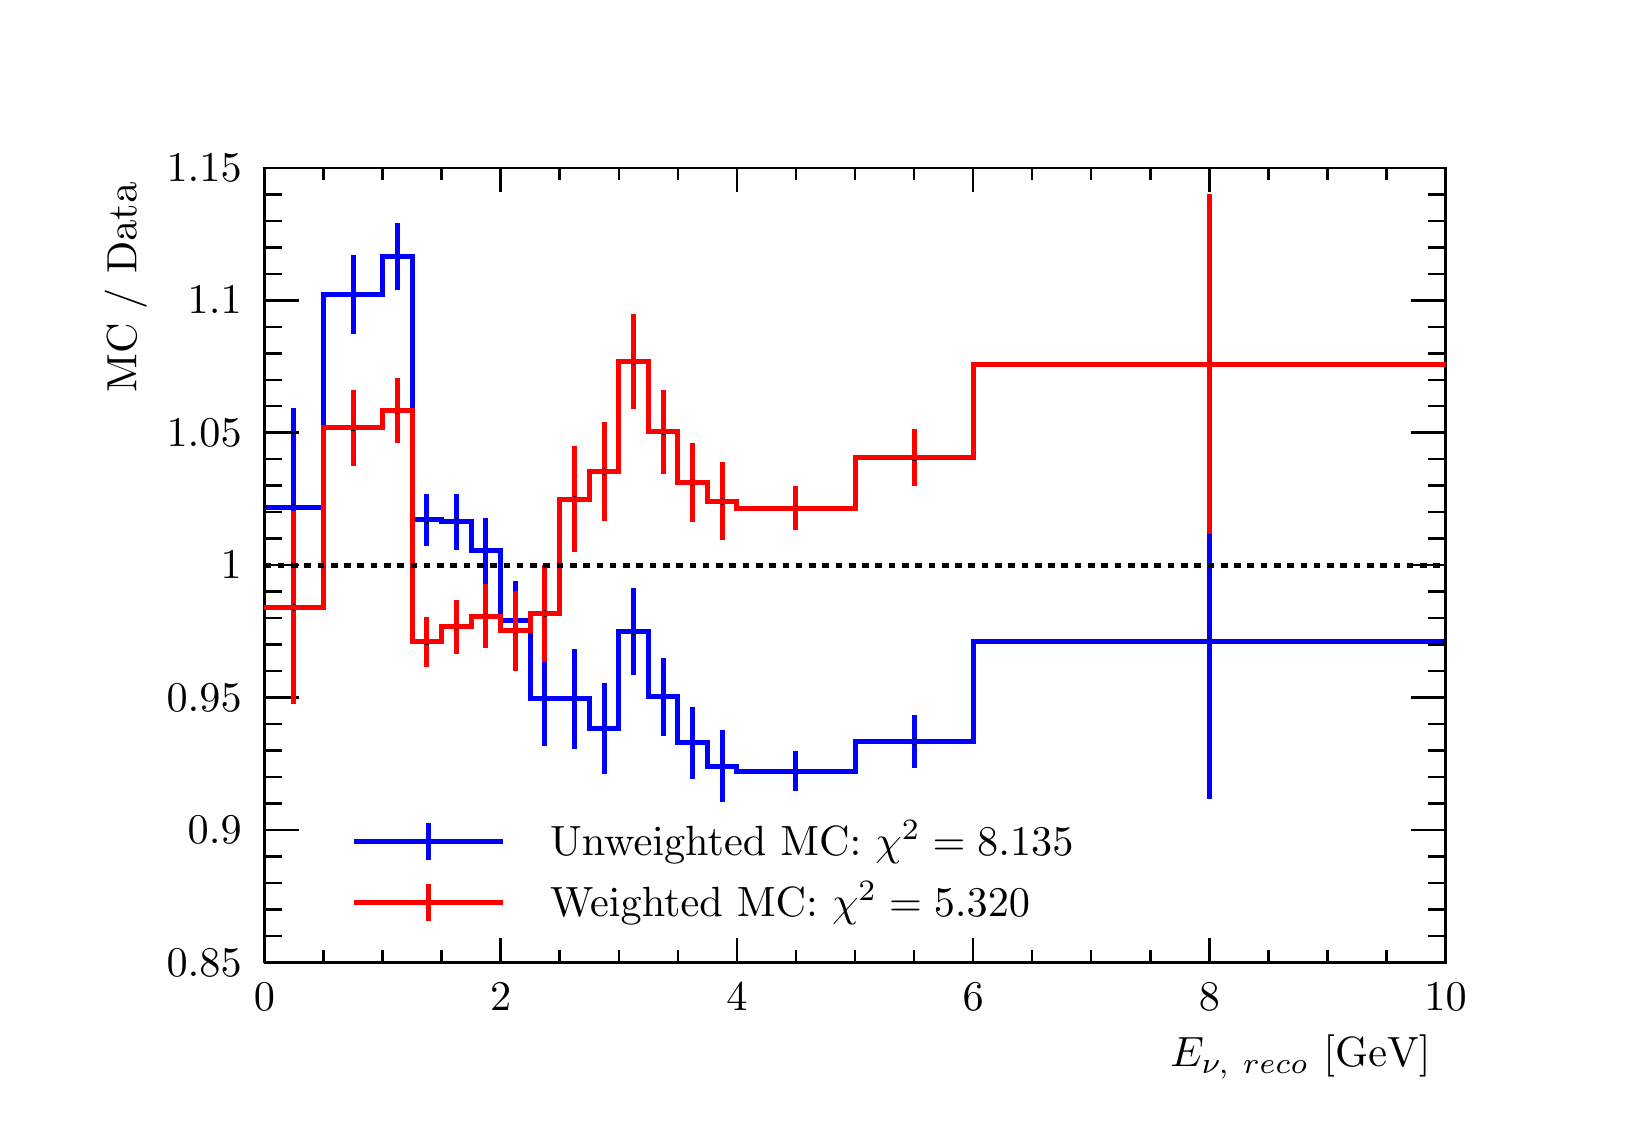
\begin{tikzpicture}
\pgfdeclareplotmark{cross} {
\pgfpathmoveto{\pgfpoint{-0.3\pgfplotmarksize}{\pgfplotmarksize}}
\pgfpathlineto{\pgfpoint{+0.3\pgfplotmarksize}{\pgfplotmarksize}}
\pgfpathlineto{\pgfpoint{+0.3\pgfplotmarksize}{0.3\pgfplotmarksize}}
\pgfpathlineto{\pgfpoint{+1\pgfplotmarksize}{0.3\pgfplotmarksize}}
\pgfpathlineto{\pgfpoint{+1\pgfplotmarksize}{-0.3\pgfplotmarksize}}
\pgfpathlineto{\pgfpoint{+0.3\pgfplotmarksize}{-0.3\pgfplotmarksize}}
\pgfpathlineto{\pgfpoint{+0.3\pgfplotmarksize}{-1.\pgfplotmarksize}}
\pgfpathlineto{\pgfpoint{-0.3\pgfplotmarksize}{-1.\pgfplotmarksize}}
\pgfpathlineto{\pgfpoint{-0.3\pgfplotmarksize}{-0.3\pgfplotmarksize}}
\pgfpathlineto{\pgfpoint{-1.\pgfplotmarksize}{-0.3\pgfplotmarksize}}
\pgfpathlineto{\pgfpoint{-1.\pgfplotmarksize}{0.3\pgfplotmarksize}}
\pgfpathlineto{\pgfpoint{-0.3\pgfplotmarksize}{0.3\pgfplotmarksize}}
\pgfpathclose
\pgfusepathqstroke
}
\pgfdeclareplotmark{cross*} {
\pgfpathmoveto{\pgfpoint{-0.3\pgfplotmarksize}{\pgfplotmarksize}}
\pgfpathlineto{\pgfpoint{+0.3\pgfplotmarksize}{\pgfplotmarksize}}
\pgfpathlineto{\pgfpoint{+0.3\pgfplotmarksize}{0.3\pgfplotmarksize}}
\pgfpathlineto{\pgfpoint{+1\pgfplotmarksize}{0.3\pgfplotmarksize}}
\pgfpathlineto{\pgfpoint{+1\pgfplotmarksize}{-0.3\pgfplotmarksize}}
\pgfpathlineto{\pgfpoint{+0.3\pgfplotmarksize}{-0.3\pgfplotmarksize}}
\pgfpathlineto{\pgfpoint{+0.3\pgfplotmarksize}{-1.\pgfplotmarksize}}
\pgfpathlineto{\pgfpoint{-0.3\pgfplotmarksize}{-1.\pgfplotmarksize}}
\pgfpathlineto{\pgfpoint{-0.3\pgfplotmarksize}{-0.3\pgfplotmarksize}}
\pgfpathlineto{\pgfpoint{-1.\pgfplotmarksize}{-0.3\pgfplotmarksize}}
\pgfpathlineto{\pgfpoint{-1.\pgfplotmarksize}{0.3\pgfplotmarksize}}
\pgfpathlineto{\pgfpoint{-0.3\pgfplotmarksize}{0.3\pgfplotmarksize}}
\pgfpathclose
\pgfusepathqfillstroke
}
\pgfdeclareplotmark{newstar} {
\pgfpathmoveto{\pgfqpoint{0pt}{\pgfplotmarksize}}
\pgfpathlineto{\pgfqpointpolar{44}{0.5\pgfplotmarksize}}
\pgfpathlineto{\pgfqpointpolar{18}{\pgfplotmarksize}}
\pgfpathlineto{\pgfqpointpolar{-20}{0.5\pgfplotmarksize}}
\pgfpathlineto{\pgfqpointpolar{-54}{\pgfplotmarksize}}
\pgfpathlineto{\pgfqpointpolar{-90}{0.5\pgfplotmarksize}}
\pgfpathlineto{\pgfqpointpolar{234}{\pgfplotmarksize}}
\pgfpathlineto{\pgfqpointpolar{198}{0.5\pgfplotmarksize}}
\pgfpathlineto{\pgfqpointpolar{162}{\pgfplotmarksize}}
\pgfpathlineto{\pgfqpointpolar{134}{0.5\pgfplotmarksize}}
\pgfpathclose
\pgfusepathqstroke
}
\pgfdeclareplotmark{newstar*} {
\pgfpathmoveto{\pgfqpoint{0pt}{\pgfplotmarksize}}
\pgfpathlineto{\pgfqpointpolar{44}{0.5\pgfplotmarksize}}
\pgfpathlineto{\pgfqpointpolar{18}{\pgfplotmarksize}}
\pgfpathlineto{\pgfqpointpolar{-20}{0.5\pgfplotmarksize}}
\pgfpathlineto{\pgfqpointpolar{-54}{\pgfplotmarksize}}
\pgfpathlineto{\pgfqpointpolar{-90}{0.5\pgfplotmarksize}}
\pgfpathlineto{\pgfqpointpolar{234}{\pgfplotmarksize}}
\pgfpathlineto{\pgfqpointpolar{198}{0.5\pgfplotmarksize}}
\pgfpathlineto{\pgfqpointpolar{162}{\pgfplotmarksize}}
\pgfpathlineto{\pgfqpointpolar{134}{0.5\pgfplotmarksize}}
\pgfpathclose
\pgfusepathqfillstroke
}
\definecolor{c}{rgb}{1,1,1};
\draw [color=c, fill=c] (0,0) rectangle (20,13.639);
\draw [color=c, fill=c] (3,1.77307) rectangle (18,11.8659);
\definecolor{c}{rgb}{0,0,0};
\draw [c,line width=0.9] (3,1.77307) -- (3,11.8659) -- (18,11.8659) -- (18,1.77307) -- (3,1.77307);
\definecolor{c}{rgb}{1,1,1};
\draw [color=c, fill=c] (3,1.77307) rectangle (18,11.8659);
\definecolor{c}{rgb}{0,0,0};
\draw [c,line width=0.9] (3,1.77307) -- (3,11.8659) -- (18,11.8659) -- (18,1.77307) -- (3,1.77307);
\definecolor{c}{rgb}{0,0,1};
\draw [c,line width=1.8] (3.375,6.29488) -- (3.375,7.55685);
\draw [c,line width=1.8] (3.375,7.55685) -- (3.375,8.81881);
\definecolor{c}{rgb}{0,0,0};
\foreach \P in {(3.375,7.55685)}{\draw[mark options={color=c,fill=c},mark size=2.402402pt, line width=0.000000pt, mark=*,mark size=1pt] plot coordinates {\P};}
\definecolor{c}{rgb}{0,0,1};
\draw [c,line width=1.8] (4.125,9.75489) -- (4.125,10.2541);
\draw [c,line width=1.8] (4.125,10.2541) -- (4.125,10.7532);
\definecolor{c}{rgb}{0,0,0};
\foreach \P in {(4.125,10.2541)}{\draw[mark options={color=c,fill=c},mark size=2.402402pt, line width=0.000000pt, mark=*,mark size=1pt] plot coordinates {\P};}
\definecolor{c}{rgb}{0,0,1};
\draw [c,line width=1.8] (4.6875,10.3081) -- (4.6875,10.7391);
\draw [c,line width=1.8] (4.6875,10.7391) -- (4.6875,11.1702);
\definecolor{c}{rgb}{0,0,0};
\foreach \P in {(4.6875,10.7391)}{\draw[mark options={color=c,fill=c},mark size=2.402402pt, line width=0.000000pt, mark=*,mark size=1pt] plot coordinates {\P};}
\definecolor{c}{rgb}{0,0,1};
\draw [c,line width=1.8] (5.0625,7.06515) -- (5.0625,7.39448);
\draw [c,line width=1.8] (5.0625,7.39448) -- (5.0625,7.72382);
\definecolor{c}{rgb}{0,0,0};
\foreach \P in {(5.0625,7.39448)}{\draw[mark options={color=c,fill=c},mark size=2.402402pt, line width=0.000000pt, mark=*,mark size=1pt] plot coordinates {\P};}
\definecolor{c}{rgb}{0,0,1};
\draw [c,line width=1.8] (5.4375,7.01789) -- (5.4375,7.37106);
\draw [c,line width=1.8] (5.4375,7.37106) -- (5.4375,7.72423);
\definecolor{c}{rgb}{0,0,0};
\foreach \P in {(5.4375,7.37106)}{\draw[mark options={color=c,fill=c},mark size=2.402402pt, line width=0.000000pt, mark=*,mark size=1pt] plot coordinates {\P};}
\definecolor{c}{rgb}{0,0,1};
\draw [c,line width=1.8] (5.8125,6.58502) -- (5.8125,7.00202);
\draw [c,line width=1.8] (5.8125,7.00202) -- (5.8125,7.41901);
\definecolor{c}{rgb}{0,0,0};
\foreach \P in {(5.8125,7.00202)}{\draw[mark options={color=c,fill=c},mark size=2.402402pt, line width=0.000000pt, mark=*,mark size=1pt] plot coordinates {\P};}
\definecolor{c}{rgb}{0,0,1};
\draw [c,line width=1.8] (6.1875,5.60236) -- (6.1875,6.11319);
\draw [c,line width=1.8] (6.1875,6.11319) -- (6.1875,6.62403);
\definecolor{c}{rgb}{0,0,0};
\foreach \P in {(6.1875,6.11319)}{\draw[mark options={color=c,fill=c},mark size=2.402402pt, line width=0.000000pt, mark=*,mark size=1pt] plot coordinates {\P};}
\definecolor{c}{rgb}{0,0,1};
\draw [c,line width=1.8] (6.5625,4.52926) -- (6.5625,5.12907);
\draw [c,line width=1.8] (6.5625,5.12907) -- (6.5625,5.72889);
\definecolor{c}{rgb}{0,0,0};
\foreach \P in {(6.5625,5.12907)}{\draw[mark options={color=c,fill=c},mark size=2.402402pt, line width=0.000000pt, mark=*,mark size=1pt] plot coordinates {\P};}
\definecolor{c}{rgb}{0,0,1};
\draw [c,line width=1.8] (6.9375,4.48615) -- (6.9375,5.12235);
\draw [c,line width=1.8] (6.9375,5.12235) -- (6.9375,5.75854);
\definecolor{c}{rgb}{0,0,0};
\foreach \P in {(6.9375,5.12235)}{\draw[mark options={color=c,fill=c},mark size=2.402402pt, line width=0.000000pt, mark=*,mark size=1pt] plot coordinates {\P};}
\definecolor{c}{rgb}{0,0,1};
\draw [c,line width=1.8] (7.3125,4.16193) -- (7.3125,4.74369);
\draw [c,line width=1.8] (7.3125,4.74369) -- (7.3125,5.32546);
\definecolor{c}{rgb}{0,0,0};
\foreach \P in {(7.3125,4.74369)}{\draw[mark options={color=c,fill=c},mark size=2.402402pt, line width=0.000000pt, mark=*,mark size=1pt] plot coordinates {\P};}
\definecolor{c}{rgb}{0,0,1};
\draw [c,line width=1.8] (7.6875,5.42015) -- (7.6875,5.9756);
\draw [c,line width=1.8] (7.6875,5.9756) -- (7.6875,6.53106);
\definecolor{c}{rgb}{0,0,0};
\foreach \P in {(7.6875,5.9756)}{\draw[mark options={color=c,fill=c},mark size=2.402402pt, line width=0.000000pt, mark=*,mark size=1pt] plot coordinates {\P};}
\definecolor{c}{rgb}{0,0,1};
\draw [c,line width=1.8] (8.0625,4.65553) -- (8.0625,5.14886);
\draw [c,line width=1.8] (8.0625,5.14886) -- (8.0625,5.64219);
\definecolor{c}{rgb}{0,0,0};
\foreach \P in {(8.0625,5.14886)}{\draw[mark options={color=c,fill=c},mark size=2.402402pt, line width=0.000000pt, mark=*,mark size=1pt] plot coordinates {\P};}
\definecolor{c}{rgb}{0,0,1};
\draw [c,line width=1.8] (8.4375,4.10305) -- (8.4375,4.56326);
\draw [c,line width=1.8] (8.4375,4.56326) -- (8.4375,5.02346);
\definecolor{c}{rgb}{0,0,0};
\foreach \P in {(8.4375,4.56326)}{\draw[mark options={color=c,fill=c},mark size=2.402402pt, line width=0.000000pt, mark=*,mark size=1pt] plot coordinates {\P};}
\definecolor{c}{rgb}{0,0,1};
\draw [c,line width=1.8] (8.8125,3.80998) -- (8.8125,4.26888);
\draw [c,line width=1.8] (8.8125,4.26888) -- (8.8125,4.72779);
\definecolor{c}{rgb}{0,0,0};
\foreach \P in {(8.8125,4.26888)}{\draw[mark options={color=c,fill=c},mark size=2.402402pt, line width=0.000000pt, mark=*,mark size=1pt] plot coordinates {\P};}
\definecolor{c}{rgb}{0,0,1};
\draw [c,line width=1.8] (9.75,3.94857) -- (9.75,4.20316);
\draw [c,line width=1.8] (9.75,4.20316) -- (9.75,4.45776);
\definecolor{c}{rgb}{0,0,0};
\foreach \P in {(9.75,4.20316)}{\draw[mark options={color=c,fill=c},mark size=2.402402pt, line width=0.000000pt, mark=*,mark size=1pt] plot coordinates {\P};}
\definecolor{c}{rgb}{0,0,1};
\draw [c,line width=1.8] (11.25,4.24636) -- (11.25,4.57969);
\draw [c,line width=1.8] (11.25,4.57969) -- (11.25,4.91302);
\definecolor{c}{rgb}{0,0,0};
\foreach \P in {(11.25,4.57969)}{\draw[mark options={color=c,fill=c},mark size=2.402402pt, line width=0.000000pt, mark=*,mark size=1pt] plot coordinates {\P};}
\definecolor{c}{rgb}{0,0,1};
\draw [c,line width=1.8] (15,3.85414) -- (15,5.85448);
\draw [c,line width=1.8] (15,5.85448) -- (15,7.85482);
\definecolor{c}{rgb}{0,0,0};
\foreach \P in {(15,5.85448)}{\draw[mark options={color=c,fill=c},mark size=2.402402pt, line width=0.000000pt, mark=*,mark size=1pt] plot coordinates {\P};}
\definecolor{c}{rgb}{0,0,1};
\draw [c,line width=1.8] (3,7.55685) -- (3.75,7.55685) -- (3.75,10.2541) -- (4.5,10.2541) -- (4.5,10.7391) -- (4.875,10.7391) -- (4.875,7.39448) -- (5.25,7.39448) -- (5.25,7.37106) -- (5.625,7.37106) -- (5.625,7.00202) -- (6,7.00202) -- (6,6.11319)
 -- (6.375,6.11319) -- (6.375,5.12907) -- (6.75,5.12907) -- (6.75,5.12235) -- (7.125,5.12235) -- (7.125,4.74369) -- (7.5,4.74369) -- (7.5,5.9756) -- (7.875,5.9756) -- (7.875,5.14886) -- (8.25,5.14886) -- (8.25,4.56326) -- (8.625,4.56326) --
 (8.625,4.26888) -- (9,4.26888) -- (9,4.20316) -- (10.5,4.20316) -- (10.5,4.57969) -- (12,4.57969) -- (12,5.85448) -- (18,5.85448);
\definecolor{c}{rgb}{0,0,0};
\draw [c,line width=0.9] (3,1.77307) -- (18,1.77307);
\draw [c,line width=0.9] (3,2.07994) -- (3,1.77307);
\draw [c,line width=0.9] (3.75,1.9265) -- (3.75,1.77307);
\draw [c,line width=0.9] (4.5,1.9265) -- (4.5,1.77307);
\draw [c,line width=0.9] (5.25,1.9265) -- (5.25,1.77307);
\draw [c,line width=0.9] (6,2.07994) -- (6,1.77307);
\draw [c,line width=0.9] (6.75,1.9265) -- (6.75,1.77307);
\draw [c,line width=0.9] (7.5,1.9265) -- (7.5,1.77307);
\draw [c,line width=0.9] (8.25,1.9265) -- (8.25,1.77307);
\draw [c,line width=0.9] (9,2.07994) -- (9,1.77307);
\draw [c,line width=0.9] (9.75,1.9265) -- (9.75,1.77307);
\draw [c,line width=0.9] (10.5,1.9265) -- (10.5,1.77307);
\draw [c,line width=0.9] (11.25,1.9265) -- (11.25,1.77307);
\draw [c,line width=0.9] (12,2.07994) -- (12,1.77307);
\draw [c,line width=0.9] (12.75,1.9265) -- (12.75,1.77307);
\draw [c,line width=0.9] (13.5,1.9265) -- (13.5,1.77307);
\draw [c,line width=0.9] (14.25,1.9265) -- (14.25,1.77307);
\draw [c,line width=0.9] (15,2.07994) -- (15,1.77307);
\draw [c,line width=0.9] (15.75,1.9265) -- (15.75,1.77307);
\draw [c,line width=0.9] (16.5,1.9265) -- (16.5,1.77307);
\draw [c,line width=0.9] (17.25,1.9265) -- (17.25,1.77307);
\draw [c,line width=0.9] (18,2.07994) -- (18,1.77307);
\draw [anchor=base] (3,1.15931) node[scale=1.52731, color=c, rotate=0]{0};
\draw [anchor=base] (6,1.15931) node[scale=1.52731, color=c, rotate=0]{2};
\draw [anchor=base] (9,1.15931) node[scale=1.52731, color=c, rotate=0]{4};
\draw [anchor=base] (12,1.15931) node[scale=1.52731, color=c, rotate=0]{6};
\draw [anchor=base] (15,1.15931) node[scale=1.52731, color=c, rotate=0]{8};
\draw [anchor=base] (18,1.15931) node[scale=1.52731, color=c, rotate=0]{10};
\draw [anchor= east] (18,0.572837) node[scale=1.52731, color=c, rotate=0]{$E_{\nu,~\text{reco}}$ [GeV]};
\draw [c,line width=0.9] (3,11.8659) -- (18,11.8659);
\draw [c,line width=0.9] (3,11.559) -- (3,11.8659);
\draw [c,line width=0.9] (3.75,11.7125) -- (3.75,11.8659);
\draw [c,line width=0.9] (4.5,11.7125) -- (4.5,11.8659);
\draw [c,line width=0.9] (5.25,11.7125) -- (5.25,11.8659);
\draw [c,line width=0.9] (6,11.559) -- (6,11.8659);
\draw [c,line width=0.9] (6.75,11.7125) -- (6.75,11.8659);
\draw [c,line width=0.9] (7.5,11.7125) -- (7.5,11.8659);
\draw [c,line width=0.9] (8.25,11.7125) -- (8.25,11.8659);
\draw [c,line width=0.9] (9,11.559) -- (9,11.8659);
\draw [c,line width=0.9] (9.75,11.7125) -- (9.75,11.8659);
\draw [c,line width=0.9] (10.5,11.7125) -- (10.5,11.8659);
\draw [c,line width=0.9] (11.25,11.7125) -- (11.25,11.8659);
\draw [c,line width=0.9] (12,11.559) -- (12,11.8659);
\draw [c,line width=0.9] (12.75,11.7125) -- (12.75,11.8659);
\draw [c,line width=0.9] (13.5,11.7125) -- (13.5,11.8659);
\draw [c,line width=0.9] (14.25,11.7125) -- (14.25,11.8659);
\draw [c,line width=0.9] (15,11.559) -- (15,11.8659);
\draw [c,line width=0.9] (15.75,11.7125) -- (15.75,11.8659);
\draw [c,line width=0.9] (16.5,11.7125) -- (16.5,11.8659);
\draw [c,line width=0.9] (17.25,11.7125) -- (17.25,11.8659);
\draw [c,line width=0.9] (18,11.559) -- (18,11.8659);
\draw [c,line width=0.9] (3,1.77307) -- (3,11.8659);
\draw [c,line width=0.9] (3.444,1.77307) -- (3,1.77307);
\draw [c,line width=0.9] (3.222,2.10949) -- (3,2.10949);
\draw [c,line width=0.9] (3.222,2.44592) -- (3,2.44592);
\draw [c,line width=0.9] (3.222,2.78235) -- (3,2.78235);
\draw [c,line width=0.9] (3.222,3.11878) -- (3,3.11878);
\draw [c,line width=0.9] (3.444,3.45521) -- (3,3.45521);
\draw [c,line width=0.9] (3.222,3.79163) -- (3,3.79163);
\draw [c,line width=0.9] (3.222,4.12806) -- (3,4.12806);
\draw [c,line width=0.9] (3.222,4.46449) -- (3,4.46449);
\draw [c,line width=0.9] (3.222,4.80092) -- (3,4.80092);
\draw [c,line width=0.9] (3.444,5.13734) -- (3,5.13734);
\draw [c,line width=0.9] (3.222,5.47377) -- (3,5.47377);
\draw [c,line width=0.9] (3.222,5.8102) -- (3,5.8102);
\draw [c,line width=0.9] (3.222,6.14663) -- (3,6.14663);
\draw [c,line width=0.9] (3.222,6.48306) -- (3,6.48306);
\draw [c,line width=0.9] (3.444,6.81948) -- (3,6.81948);
\draw [c,line width=0.9] (3.222,7.15591) -- (3,7.15591);
\draw [c,line width=0.9] (3.222,7.49234) -- (3,7.49234);
\draw [c,line width=0.9] (3.222,7.82877) -- (3,7.82877);
\draw [c,line width=0.9] (3.222,8.1652) -- (3,8.1652);
\draw [c,line width=0.9] (3.444,8.50162) -- (3,8.50162);
\draw [c,line width=0.9] (3.222,8.83805) -- (3,8.83805);
\draw [c,line width=0.9] (3.222,9.17448) -- (3,9.17448);
\draw [c,line width=0.9] (3.222,9.51091) -- (3,9.51091);
\draw [c,line width=0.9] (3.222,9.84733) -- (3,9.84733);
\draw [c,line width=0.9] (3.444,10.1838) -- (3,10.1838);
\draw [c,line width=0.9] (3.222,10.5202) -- (3,10.5202);
\draw [c,line width=0.9] (3.222,10.8566) -- (3,10.8566);
\draw [c,line width=0.9] (3.222,11.193) -- (3,11.193);
\draw [c,line width=0.9] (3.222,11.5295) -- (3,11.5295);
\draw [c,line width=0.9] (3.444,11.8659) -- (3,11.8659);
\draw [c,line width=0.9] (3.444,1.77307) -- (3,1.77307);
\draw [c,line width=0.9] (3.444,11.8659) -- (3,11.8659);
\draw [anchor= east] (2.9,1.77307) node[scale=1.52731, color=c, rotate=0]{0.85};
\draw [anchor= east] (2.9,3.45521) node[scale=1.52731, color=c, rotate=0]{0.9};
\draw [anchor= east] (2.9,5.13734) node[scale=1.52731, color=c, rotate=0]{0.95};
\draw [anchor= east] (2.9,6.81948) node[scale=1.52731, color=c, rotate=0]{1};
\draw [anchor= east] (2.9,8.50162) node[scale=1.52731, color=c, rotate=0]{1.05};
\draw [anchor= east] (2.9,10.1838) node[scale=1.52731, color=c, rotate=0]{1.1};
\draw [anchor= east] (2.9,11.8659) node[scale=1.52731, color=c, rotate=0]{1.15};
\draw [anchor= east] (1.24,11.8659) node[scale=1.52731, color=c, rotate=90]{MC / Data};
\draw [c,line width=0.9] (18,1.77307) -- (18,11.8659);
\draw [c,line width=0.9] (17.556,1.77307) -- (18,1.77307);
\draw [c,line width=0.9] (17.778,2.10949) -- (18,2.10949);
\draw [c,line width=0.9] (17.778,2.44592) -- (18,2.44592);
\draw [c,line width=0.9] (17.778,2.78235) -- (18,2.78235);
\draw [c,line width=0.9] (17.778,3.11878) -- (18,3.11878);
\draw [c,line width=0.9] (17.556,3.45521) -- (18,3.45521);
\draw [c,line width=0.9] (17.778,3.79163) -- (18,3.79163);
\draw [c,line width=0.9] (17.778,4.12806) -- (18,4.12806);
\draw [c,line width=0.9] (17.778,4.46449) -- (18,4.46449);
\draw [c,line width=0.9] (17.778,4.80092) -- (18,4.80092);
\draw [c,line width=0.9] (17.556,5.13734) -- (18,5.13734);
\draw [c,line width=0.9] (17.778,5.47377) -- (18,5.47377);
\draw [c,line width=0.9] (17.778,5.8102) -- (18,5.8102);
\draw [c,line width=0.9] (17.778,6.14663) -- (18,6.14663);
\draw [c,line width=0.9] (17.778,6.48306) -- (18,6.48306);
\draw [c,line width=0.9] (17.556,6.81948) -- (18,6.81948);
\draw [c,line width=0.9] (17.778,7.15591) -- (18,7.15591);
\draw [c,line width=0.9] (17.778,7.49234) -- (18,7.49234);
\draw [c,line width=0.9] (17.778,7.82877) -- (18,7.82877);
\draw [c,line width=0.9] (17.778,8.1652) -- (18,8.1652);
\draw [c,line width=0.9] (17.556,8.50162) -- (18,8.50162);
\draw [c,line width=0.9] (17.778,8.83805) -- (18,8.83805);
\draw [c,line width=0.9] (17.778,9.17448) -- (18,9.17448);
\draw [c,line width=0.9] (17.778,9.51091) -- (18,9.51091);
\draw [c,line width=0.9] (17.778,9.84733) -- (18,9.84733);
\draw [c,line width=0.9] (17.556,10.1838) -- (18,10.1838);
\draw [c,line width=0.9] (17.778,10.5202) -- (18,10.5202);
\draw [c,line width=0.9] (17.778,10.8566) -- (18,10.8566);
\draw [c,line width=0.9] (17.778,11.193) -- (18,11.193);
\draw [c,line width=0.9] (17.778,11.5295) -- (18,11.5295);
\draw [c,line width=0.9] (17.556,11.8659) -- (18,11.8659);
\draw [c,line width=0.9] (17.556,1.77307) -- (18,1.77307);
\draw [c,line width=0.9] (17.556,11.8659) -- (18,11.8659);
\definecolor{c}{rgb}{1,0,0};
\draw [c,line width=1.8] (3.375,5.05805) -- (3.375,6.28481);
\draw [c,line width=1.8] (3.375,6.28481) -- (3.375,7.51158);
\definecolor{c}{rgb}{0,0,0};
\foreach \P in {(3.375,6.28481)}{\draw[mark options={color=c,fill=c},mark size=2.402402pt, line width=0.000000pt, mark=*,mark size=1pt] plot coordinates {\P};}
\definecolor{c}{rgb}{1,0,0};
\draw [c,line width=1.8] (4.125,8.08125) -- (4.125,8.56304);
\draw [c,line width=1.8] (4.125,8.56304) -- (4.125,9.04482);
\definecolor{c}{rgb}{0,0,0};
\foreach \P in {(4.125,8.56304)}{\draw[mark options={color=c,fill=c},mark size=2.402402pt, line width=0.000000pt, mark=*,mark size=1pt] plot coordinates {\P};}
\definecolor{c}{rgb}{1,0,0};
\draw [c,line width=1.8] (4.6875,8.365) -- (4.6875,8.77886);
\draw [c,line width=1.8] (4.6875,8.77886) -- (4.6875,9.19271);
\definecolor{c}{rgb}{0,0,0};
\foreach \P in {(4.6875,8.77886)}{\draw[mark options={color=c,fill=c},mark size=2.402402pt, line width=0.000000pt, mark=*,mark size=1pt] plot coordinates {\P};}
\definecolor{c}{rgb}{1,0,0};
\draw [c,line width=1.8] (5.0625,5.52706) -- (5.0625,5.84516);
\draw [c,line width=1.8] (5.0625,5.84516) -- (5.0625,6.16325);
\definecolor{c}{rgb}{0,0,0};
\foreach \P in {(5.0625,5.84516)}{\draw[mark options={color=c,fill=c},mark size=2.402402pt, line width=0.000000pt, mark=*,mark size=1pt] plot coordinates {\P};}
\definecolor{c}{rgb}{1,0,0};
\draw [c,line width=1.8] (5.4375,5.69391) -- (5.4375,6.0367);
\draw [c,line width=1.8] (5.4375,6.0367) -- (5.4375,6.37949);
\definecolor{c}{rgb}{0,0,0};
\foreach \P in {(5.4375,6.0367)}{\draw[mark options={color=c,fill=c},mark size=2.402402pt, line width=0.000000pt, mark=*,mark size=1pt] plot coordinates {\P};}
\definecolor{c}{rgb}{1,0,0};
\draw [c,line width=1.8] (5.8125,5.76368) -- (5.8125,6.17299);
\draw [c,line width=1.8] (5.8125,6.17299) -- (5.8125,6.58231);
\definecolor{c}{rgb}{0,0,0};
\foreach \P in {(5.8125,6.17299)}{\draw[mark options={color=c,fill=c},mark size=2.402402pt, line width=0.000000pt, mark=*,mark size=1pt] plot coordinates {\P};}
\definecolor{c}{rgb}{1,0,0};
\draw [c,line width=1.8] (6.1875,5.47714) -- (6.1875,5.9865);
\draw [c,line width=1.8] (6.1875,5.9865) -- (6.1875,6.49587);
\definecolor{c}{rgb}{0,0,0};
\foreach \P in {(6.1875,5.9865)}{\draw[mark options={color=c,fill=c},mark size=2.402402pt, line width=0.000000pt, mark=*,mark size=1pt] plot coordinates {\P};}
\definecolor{c}{rgb}{1,0,0};
\draw [c,line width=1.8] (6.5625,5.59326) -- (6.5625,6.20812);
\draw [c,line width=1.8] (6.5625,6.20812) -- (6.5625,6.82297);
\definecolor{c}{rgb}{0,0,0};
\foreach \P in {(6.5625,6.20812)}{\draw[mark options={color=c,fill=c},mark size=2.402402pt, line width=0.000000pt, mark=*,mark size=1pt] plot coordinates {\P};}
\definecolor{c}{rgb}{1,0,0};
\draw [c,line width=1.8] (6.9375,6.98489) -- (6.9375,7.65852);
\draw [c,line width=1.8] (6.9375,7.65852) -- (6.9375,8.33214);
\definecolor{c}{rgb}{0,0,0};
\foreach \P in {(6.9375,7.65852)}{\draw[mark options={color=c,fill=c},mark size=2.402402pt, line width=0.000000pt, mark=*,mark size=1pt] plot coordinates {\P};}
\definecolor{c}{rgb}{1,0,0};
\draw [c,line width=1.8] (7.3125,7.38229) -- (7.3125,8.00851);
\draw [c,line width=1.8] (7.3125,8.00851) -- (7.3125,8.63473);
\definecolor{c}{rgb}{0,0,0};
\foreach \P in {(7.3125,8.00851)}{\draw[mark options={color=c,fill=c},mark size=2.402402pt, line width=0.000000pt, mark=*,mark size=1pt] plot coordinates {\P};}
\definecolor{c}{rgb}{1,0,0};
\draw [c,line width=1.8] (7.6875,8.80856) -- (7.6875,9.40723);
\draw [c,line width=1.8] (7.6875,9.40723) -- (7.6875,10.0059);
\definecolor{c}{rgb}{0,0,0};
\foreach \P in {(7.6875,9.40723)}{\draw[mark options={color=c,fill=c},mark size=2.402402pt, line width=0.000000pt, mark=*,mark size=1pt] plot coordinates {\P};}
\definecolor{c}{rgb}{1,0,0};
\draw [c,line width=1.8] (8.0625,7.98357) -- (8.0625,8.51536);
\draw [c,line width=1.8] (8.0625,8.51536) -- (8.0625,9.04714);
\definecolor{c}{rgb}{0,0,0};
\foreach \P in {(8.0625,8.51536)}{\draw[mark options={color=c,fill=c},mark size=2.402402pt, line width=0.000000pt, mark=*,mark size=1pt] plot coordinates {\P};}
\definecolor{c}{rgb}{1,0,0};
\draw [c,line width=1.8] (8.4375,7.37314) -- (8.4375,7.86912);
\draw [c,line width=1.8] (8.4375,7.86912) -- (8.4375,8.3651);
\definecolor{c}{rgb}{0,0,0};
\foreach \P in {(8.4375,7.86912)}{\draw[mark options={color=c,fill=c},mark size=2.402402pt, line width=0.000000pt, mark=*,mark size=1pt] plot coordinates {\P};}
\definecolor{c}{rgb}{1,0,0};
\draw [c,line width=1.8] (8.8125,7.13347) -- (8.8125,7.62892);
\draw [c,line width=1.8] (8.8125,7.62892) -- (8.8125,8.12436);
\definecolor{c}{rgb}{0,0,0};
\foreach \P in {(8.8125,7.62892)}{\draw[mark options={color=c,fill=c},mark size=2.402402pt, line width=0.000000pt, mark=*,mark size=1pt] plot coordinates {\P};}
\definecolor{c}{rgb}{1,0,0};
\draw [c,line width=1.8] (9.75,7.26987) -- (9.75,7.54465);
\draw [c,line width=1.8] (9.75,7.54465) -- (9.75,7.81944);
\definecolor{c}{rgb}{0,0,0};
\foreach \P in {(9.75,7.54465)}{\draw[mark options={color=c,fill=c},mark size=2.402402pt, line width=0.000000pt, mark=*,mark size=1pt] plot coordinates {\P};}
\definecolor{c}{rgb}{1,0,0};
\draw [c,line width=1.8] (11.25,7.82103) -- (11.25,8.18258);
\draw [c,line width=1.8] (11.25,8.18258) -- (11.25,8.54414);
\definecolor{c}{rgb}{0,0,0};
\foreach \P in {(11.25,8.18258)}{\draw[mark options={color=c,fill=c},mark size=2.402402pt, line width=0.000000pt, mark=*,mark size=1pt] plot coordinates {\P};}
\definecolor{c}{rgb}{1,0,0};
\draw [c,line width=1.8] (15,7.21212) -- (15,9.3725);
\draw [c,line width=1.8] (15,9.3725) -- (15,11.5329);
\definecolor{c}{rgb}{0,0,0};
\foreach \P in {(15,9.3725)}{\draw[mark options={color=c,fill=c},mark size=2.402402pt, line width=0.000000pt, mark=*,mark size=1pt] plot coordinates {\P};}
\definecolor{c}{rgb}{1,0,0};
\draw [c,line width=1.8] (3,6.28481) -- (3.75,6.28481) -- (3.75,8.56304) -- (4.5,8.56304) -- (4.5,8.77886) -- (4.875,8.77886) -- (4.875,5.84516) -- (5.25,5.84516) -- (5.25,6.0367) -- (5.625,6.0367) -- (5.625,6.17299) -- (6,6.17299) -- (6,5.9865) --
 (6.375,5.9865) -- (6.375,6.20812) -- (6.75,6.20812) -- (6.75,7.65852) -- (7.125,7.65852) -- (7.125,8.00851) -- (7.5,8.00851) -- (7.5,9.40723) -- (7.875,9.40723) -- (7.875,8.51536) -- (8.25,8.51536) -- (8.25,7.86912) -- (8.625,7.86912) --
 (8.625,7.62892) -- (9,7.62892) -- (9,7.54465) -- (10.5,7.54465) -- (10.5,8.18258) -- (12,8.18258) -- (12,9.3725) -- (18,9.3725);
\definecolor{c}{rgb}{0,0,0};
\draw [c,dash pattern=on 2.40pt off 2.40pt ,line width=1.8] (3,6.81948) -- (18,6.81948);
\definecolor{c}{rgb}{1,1,1};
\draw [color=c, fill=c] (3.72493,2.149) rectangle (14.5845,3.69627);
\definecolor{c}{rgb}{0,0,0};
\draw [anchor=base west] (6.43983,3.13539) node[scale=1.52731, color=c, rotate=0]{Unweighted MC: $\chi^{2} = 8.135$};
\definecolor{c}{rgb}{0,0,1};
\draw [c,line width=1.8] (4.13216,3.30946) -- (6.03259,3.30946);
\draw [c,line width=1.8] (5.08238,3.07736) -- (5.08238,3.54155);
\definecolor{c}{rgb}{0,0,0};
\draw [anchor=base west] (6.43983,2.36175) node[scale=1.52731, color=c, rotate=0]{Weighted MC: $\chi^{2} = 5.320$};
\definecolor{c}{rgb}{1,0,0};
\draw [c,line width=1.8] (4.13216,2.53582) -- (6.03259,2.53582);
\draw [c,line width=1.8] (5.08238,2.30373) -- (5.08238,2.76791);
\definecolor{c}{rgb}{1,1,1};
\draw [color=c, fill=c] (2,12.8206) rectangle (18,13.5708);
\end{tikzpicture}
